% $Header: /cvsroot/latex-beamer/latex-beamer/solutions/generic-talks/generic-ornate-15min-45min.en.tex,v 1.5 2007/01/28 20:48:23 tantau Exp $

\documentclass{beamer}

% This file is a solution template for:

% - Giving a talk on some subject.
% - The talk is between 15min and 45min long.
% - Style is ornate.



% Copyright 2004 by Till Tantau <tantau@users.sourceforge.net>.
%
% In principle, this file can be redistributed and/or modified under
% the terms of the GNU Public License, version 2.
%
% However, this file is supposed to be a template to be modified
% for your own needs. For this reason, if you use this file as a
% template and not specifically distribute it as part of a another
% package/program, I grant the extra permission to freely copy and
% modify this file as you see fit and even to delete this copyright
% notice. 


\mode<presentation>
{
	\usetheme{Warsaw}
	% or ...

		\setbeamercovered{transparent}
	% or whatever (possibly just delete it)
}


\usepackage[english]{babel}
% or whatever

\usepackage[latin1]{inputenc}
% or whatever

\usepackage{times}
\usepackage[T1]{fontenc}
% Or whatever. Note that the encoding and the font should match. If T1
% does not look nice, try deleting the line with the fontenc.


\title[Project Title] % (optional, use only with long paper titles)
{Graduate Student Information System (gSIMS) }

	\subtitle
{Walkthrough} % (optional)

\author[Author] % (optional, use only with lots of authors)
{Kartik Thakore\inst{1}}
% - Use the \inst{?} command only if the authors have different
%   affiliation.

\institute[University Information] % (optional, but mostly needed)
{
	\inst{1}%
		Department of Software Engineering\\
		University of Western Ontario
}
% - Use the \inst command only if there are several affiliations.
% - Keep it simple, no one is interested in your street address.

\date[Date] % (optional)
{23 Nov 2010}

\subject{Talks}
% This is only inserted into the PDF information catalog. Can be left
% out. 



% If you have a file called "university-logo-filename.xxx", where xxx
% is a graphic format that can be processed by latex or pdflatex,
	% resp., then you can add a logo as follows:

	\pgfdeclareimage[height=0.5cm]{university-logo}{university-logo-filename}
	\logo{\pgfuseimage{university-logo}}



	% Delete this, if you do not want the table of contents to pop up at
	% the beginning of each subsection:
	\AtBeginSubsection[]
{
	\begin{frame}<beamer>{Outline}
	\tableofcontents[currentsection,currentsubsection]
		\end{frame}
}


% If you wish to uncover everything in a step-wise fashion, uncomment
% the following command: 

%\beamerdefaultoverlayspecification{<+->}


\begin{document}

\begin{frame}
\titlepage
\end{frame}

\begin{frame}{Outline}
\tableofcontents
% You might wish to add the option [pausesections]
\end{frame}


% Since this a solution template for a generic talk, very little can
% be said about how it should be structured. However, the talk length
% of between 15min and 45min and the theme suggest that you stick to
% the following rules:  

% - Exactly two or three sections (other than the summary).
% - At *most* three subsections per section.
% - Talk about 30s to 2min per frame. So there should be between about
%   15 and 30 frames, all told.

\section{Introduction}

\subsection[Project Details]{Project Details}
\begin{frame}{Project Inception}
% - A title should summarize the slide in an understandable fashion
%   for anyone how does not follow everything on the slide itself.

\begin{itemize}
\item
Advisor: Dr. Hanif Ladak
\item
Concerned with managing students in the graduate program for BioMedical Physics.
\item 
Current system has lots of problems.
\begin{itemize}
\item 
Calculations and updates are mostly manual.
\item
Need to keep the paper copies of meetings.
\item 
Takes lots of time to create reports.
\item 
Hard to track when a student must have a requirement done.
\end{itemize}
\end{itemize}
\end{frame}
\begin{frame}{Current System}
Demo of the Current System.
\end{frame}


\begin{frame}{Project Organization}

Two components of the problem:
\begin{itemize}
\item
(ECE4416) Business rules:
\begin{itemize}
\item
Graduate program milestones and dataflow.
\item
Direct interaction with the User.
\end{itemize}
\item 
(SE4450) Technical requirements:
\begin{itemize}
\item
Provide the functionality for the User Interfaces.
\item 
Adhere to required constraints.
\end{itemize}
\end{itemize}



\end{frame}
\begin{frame}{Proposal}

\begin{figure}
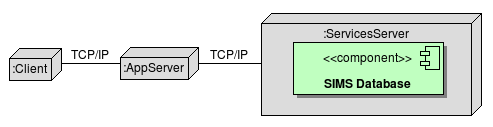
\includegraphics[width=261px]{images/scope} \caption{ The proposed system }
\end{figure}

\end{frame}
\section{Requirements}

\subsection{Technical Requirements}

\begin{frame}{Interfaces}
\begin{itemize}
\item 
Graphical User Interface:
\begin{itemize}
\item 
The implementation of the Business Rules defined as HTML pages. 
\end{itemize}
\item 
Electrical User Interface:
	\begin{itemize}
	\item 
	Collect signatures from a Wacom \copyright Tablet and store securely in the DataBase.
	\end{itemize}
\end{itemize}
\end{frame}

\begin{frame}{Graphical User Interface}
Specific requirements for the view of the Web Pages:
\begin{itemize}
\item 
Set of HTML pages that are to be the template of the system.
\begin{figure}
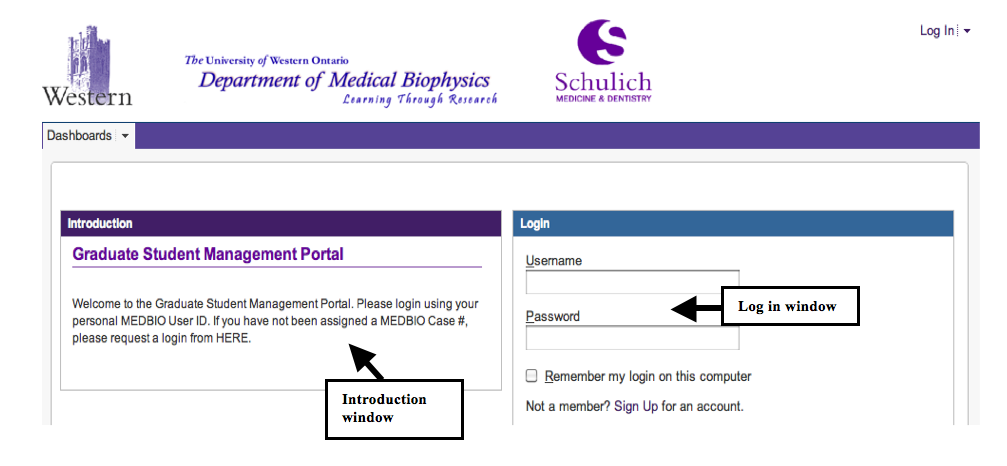
\includegraphics[width=180px]{images/ht/LogIn.png} \caption{ Sample GUI provided }
\end{figure}
\end{itemize}
\end{frame}


\begin{frame}{Electrical Device Interface}
\begin{itemize}
\item
Provide an interface for the User to sign on the screen.
\item
On the client side acquire a bitmap of the signature and encrypt the bitmap data.
\item 
The image should be viewable only by the user who signed and the graduate admin.
\end{itemize}
\end{frame}

\begin{frame}{System Features}
\begin{itemize}
\item
User Administration
\item
Tracking Data
\begin{itemize}
\item
Student Data
\item
Student Term and Funding Data
\item 
Student Program Data
\item 
Student Advisory Commitee Meeting 
\end{itemize}
\item 
Reporting
\begin{itemize}
\item
Customized Queries
\item 
Student Output Reports
\end{itemize}
\item
Triggering System 
\end{itemize}
\end{frame}

\begin{frame}{Constraints}
\begin{itemize}
\item 
Security 
\begin{itemize}
\item 
System Security
\item
Roles and Operational Access
\end{itemize}
\begin{figure}[!h]
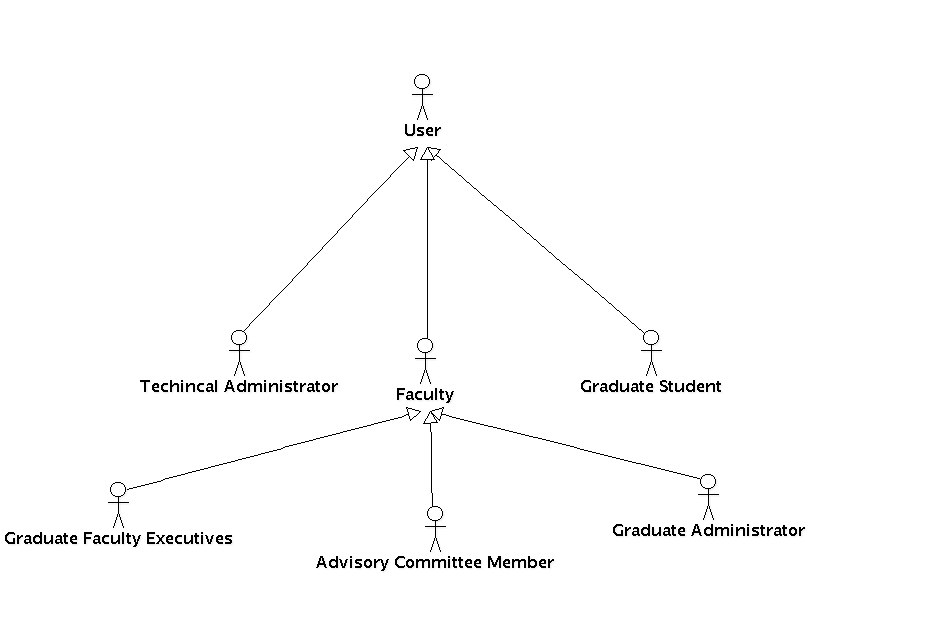
\includegraphics[width=180px]{diagrams/use_cases/UserHeirachy_uc} \caption{ Roles of the SIMS system } \label{fig:Users}
\end{figure}
\end{itemize}
\end{frame}
\section{Architectural Analysis}

\subsection{Analysis}
\begin{frame}{Organizing Data}
\begin{itemize}
\item
Seperate Authentication Data from Critical Data
\begin{figure}[!h]
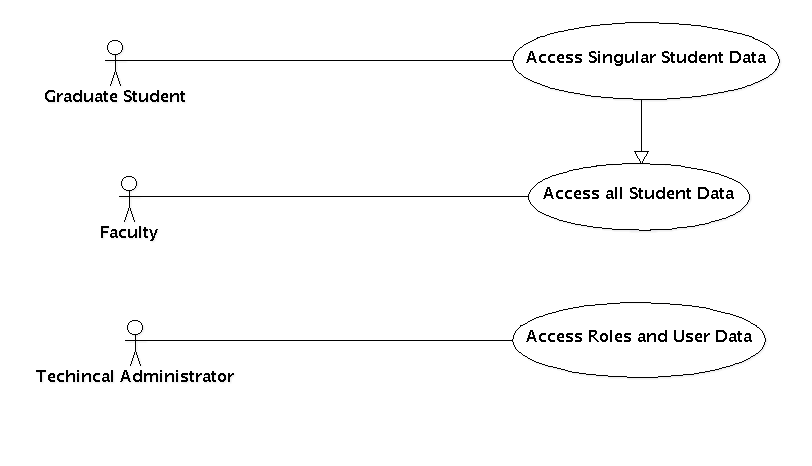
\includegraphics[width=206px]{diagrams/use_cases/seperation_of_data_uc.png} \caption{ 3 general data use cases } \label{fig:Users}
\end{figure}

\end{itemize}
\end{frame}
\begin{frame}{Conceptual Model of the Student}
\begin{itemize}
\item
Student can be treated as a ticket, which needs to go through steps to be completed.
\begin{figure}[!h]
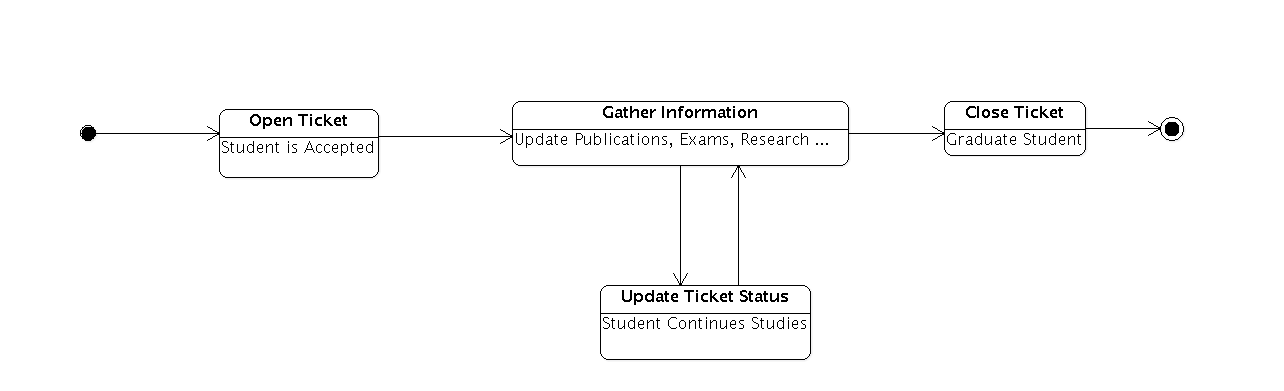
\includegraphics[width=319px]{diagrams/state_chart/student_ticket.png} \caption{ The simple steps of Grad School } \label{fig:Users}
\end{figure}
\end{itemize}
\end{frame}
\begin{frame}{Critical Assumptions}
\begin{itemize}
\item Seperation of Data
\begin{itemize}
\item
Student Data is kept around even after student has graduated.
\end{itemize}
\item Student as a Bug Ticket
\begin{itemize}
\item
Student will be responsible for their own data.
\item
Student can only be a student if they have a funded term.
\end{itemize}
\item
Data entry will be done manually at this point.
\end{itemize}
\end{frame}

\subsection{Architecture}
\begin{frame}{Hardware}
\begin{itemize}
\item Clients
\item Application Server
\item Services Server
\begin{figure}[!h]
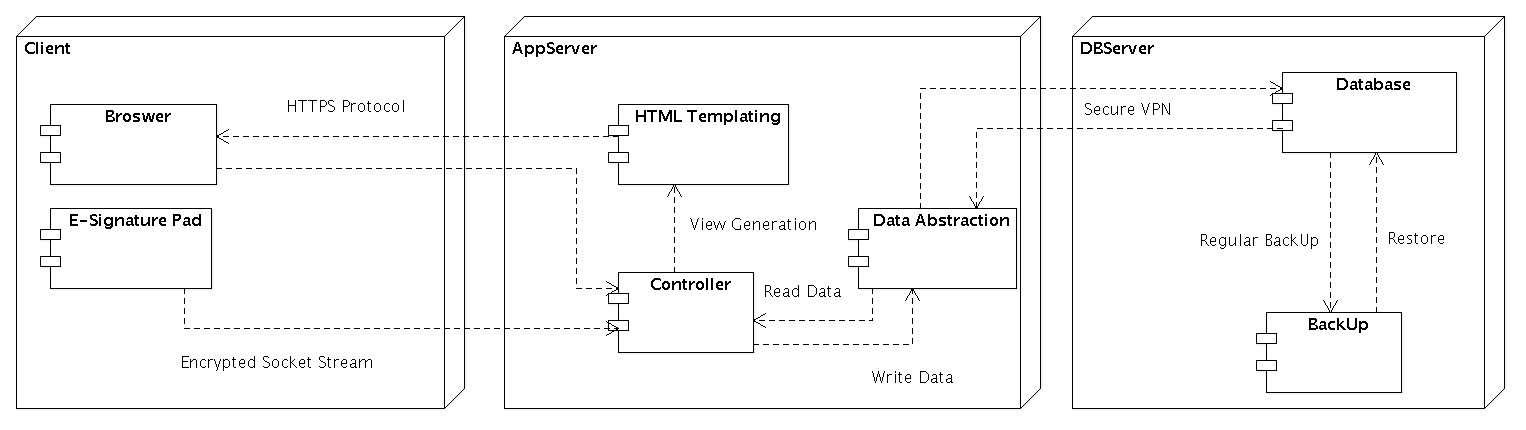
\includegraphics[width=180px]{diagrams/SystemOverview.png} \caption{ The System Overview } \label{fig:Users}
\end{figure}

\end{itemize}
\end{frame}
\begin{frame}{Software}
\begin{itemize}
\item E-Signature Capture Client
\item OpenVPN Server
\item Production HTTP server
\item Database Server
\item Perl Modules 
\end{itemize}
\end{frame}
\section{Iterative Design}

\subsection{Iteration 1}
\begin{frame}{Rapid Protoyping}
\begin{itemize}
\item Perl Framework
\item Database Schema
\item E-Signature client
\end{itemize}
\end{frame}

\begin{frame}{Test Plans}
\begin{itemize}
\item Unit Tests
\item Integration Testing
\item System Integration testing
\end{itemize}
\end{frame}





\section*{Summary}

\begin{frame}{Summary}

% Keep the summary *very short*.
\begin{itemize}
\item
Requirements and Analysis has received direct user feedback.
\item
Architecture based of the Analysis has been clarified and prototyped. 
\item 
The iterative Software Life Cycle has produced useful work quickly and with less effort.
\item
An emphasis on testing levels is present from the starting.
\end{itemize}
\end{frame}


\end{document}


